\documentclass[conference]{IEEEtran}
\IEEEoverridecommandlockouts

\usepackage{cite}
\usepackage{graphicx}
\usepackage{booktabs}
\usepackage{array}
\usepackage{multirow}
\usepackage{url}
\usepackage{amsmath}
\usepackage{textcomp}
\usepackage{xcolor}
\usepackage{caption}
\captionsetup{font=small}

\def\BibTeX{{\rm B\kern-.05em{\sc i\kern-.025em b}\kern-.08em
    T\kern-.1667em\lower.7ex\hbox{E}\kern-.125emX}}

\begin{document}

\title{Automating Continuous Compliance in DevSecOps Through Zero Trust: A Kubernetes Microservices Reference Implementation}

\author{
\IEEEauthorblockN{EMIM Ekanayaka}
\IEEEauthorblockA{
Master of Information Security (MIS) \\
University of Colombo School of Computing (UCSC) \\
Colombo, Sri Lanka
}
}

\maketitle

\begin{abstract}
Cloud-native application development has transformed how organisations build and operate software systems, but the rapid adoption of Kubernetes-based microservices has outpaced traditional approaches for verifying infrastructure, application, and runtime security controls. Perimeter-based security models, which rely on implicit trust within network boundaries, are incompatible with the dynamic and distributed nature of containerised environments, leaving security and compliance processes fragmented across tools and lifecycle stages. Although Zero Trust Architecture (ZTA), DevSecOps, and Kubernetes security have each been studied extensively, existing work largely addresses individual security domains in isolation, with limited evidence of end-to-end frameworks that operationalise Zero Trust across the full Kubernetes delivery lifecycle. This paper addresses that gap by designing, implementing, and evaluating a Zero-Trust DevSecOps framework for a Kubernetes-based microservices application, FreshBonds. Using the Design Science Research Methodology (DSRM), we develop a six-layer security architecture that integrates infrastructure as code, GitOps-driven deployment, dual-engine policy-as-code enforcement, container vulnerability scanning, automated secret lifecycle management, eBPF-based runtime threat detection, and AI-assisted incident enrichment. The framework is deployed on a production-grade three-node Kubernetes cluster on Oracle Cloud Infrastructure. Evaluation against NIST SP 800-207, pipeline security-gate testing, policy coverage analysis, runtime detection assessment, and MITRE ATT\&CK for Containers coverage analysis shows alignment with all seven NIST Zero Trust tenets, integration of ten security tools across six CI/CD pipelines, enforcement of thirty-nine policy and runtime rules, and detection coverage of thirteen MITRE ATT\&CK techniques across eight of twelve tactics. Controlled experiments confirm that CI/CD security gates block deployments containing critical vulnerabilities and policy violations, while injected runtime events are detected and enriched in near real time. These results demonstrate that continuous compliance can be operationalised as a set of automated control points distributed across the delivery lifecycle rather than as a periodic manual audit, and the paper contributes a reproducible, open-source reference implementation that bridges Zero Trust theory and practical DevSecOps adoption for Kubernetes.
\end{abstract}

\begin{IEEEkeywords}
Zero Trust Architecture, DevSecOps, continuous compliance, Kubernetes, GitOps, policy as code, Falco, eBPF, Kyverno, Open Policy Agent, MITRE ATT\&CK, AI-assisted security monitoring
\end{IEEEkeywords}

\section{Introduction}

The adoption of cloud-native technologies has accelerated dramatically across the software industry. The Cloud Native Computing Foundation (CNCF) Annual Survey 2024 reports that over ninety-six per cent of organisations are now using or evaluating Kubernetes \cite{cncf2024}, which has become the de facto standard for container orchestration, enabling organisations to deploy, scale, and manage microservice architectures at unprecedented speed \cite{burns2016}. This velocity introduces a fundamental security paradox: the ephemeral, distributed, and highly automated characteristics that make cloud-native systems attractive also render traditional, perimeter-based security models inadequate.

Perimeter-based security assumes that entities inside a network boundary can be implicitly trusted \cite{kindervag2010}. In a Kubernetes environment this assumption breaks down for several reasons. Containers are ephemeral, with pods created, destroyed, and rescheduled continuously, so their identity and network location are not stable trust anchors. Microservices communicate over internal cluster networks where east-west traffic is frequently unmonitored and unencrypted. The software supply chain introduces transitive dependencies from public registries and base images that may carry known or unknown vulnerabilities \cite{sonatype2023}. Finally, the DevOps velocity model compresses the window in which security controls can be applied and verified.

Industry evidence supports the scale of the problem: the Red Hat \emph{State of Kubernetes Security Report 2024} found that sixty-seven per cent of organisations had delayed deployment due to security concerns, and forty-six per cent had experienced a security incident in their container or Kubernetes environment in the preceding twelve months \cite{redhat2024}. The report attributes this to fragmentation -- security tooling exists, but it is scattered across pipeline stages and teams, without the automation needed to keep pace with deployment frequency.

Zero Trust Architecture (ZTA), as defined in NIST Special Publication 800-207, offers a conceptual response: it replaces implicit network trust with a principle of ``never trust, always verify,'' requiring every request, identity, and resource access to be authenticated, authorised, and continuously validated regardless of network location \cite{rose2020}. NIST SP 800-207 defines seven tenets spanning resource identification, communication security, per-session access, dynamic policy, continuous monitoring, strict enforcement, and continuous posture improvement. Translating these tenets into concrete, automated Kubernetes controls, however, remains an open engineering and research problem. DevSecOps complements ZTA by embedding security as a first-class concern throughout the software delivery lifecycle rather than as a final gate \cite{myrbakken2017}, but shift-left security alone is insufficient: controls are also required at deployment time (admission policy), at runtime (kernel-level monitoring), and post-deployment (continuous rescanning and secret rotation).

This study addresses the resulting research problem: organisations deploying Kubernetes microservices face fragmented security and compliance landscapes with limited integration across development, deployment, and runtime stages, and there is limited practical guidance on operationalising Zero Trust principles as automated, verifiable controls within a DevSecOps pipeline. We design, implement, and evaluate a Zero-Trust DevSecOps framework for a Kubernetes-based microservices application, \emph{FreshBonds}, using the Design Science Research Methodology \cite{hevner2004,peffers2007}. The contributions of this paper are:
\begin{itemize}
\item a six-layer, defence-in-depth reference architecture that maps NIST SP 800-207 tenets to concrete infrastructure, platform, application, CI/CD, runtime, and observability controls;
\item a dual-engine policy-as-code design combining Kyverno and Open Policy Agent (OPA) with eBPF-based runtime detection (Falco), evaluated against the MITRE ATT\&CK for Containers matrix;
\item an automated secret lifecycle and CI/CD security-gate design with reproducible, Git-based audit evidence; and
\item an evidence-based evaluation, including controlled fault-injection experiments, that maps repository artefacts to NIST Zero Trust tenets and quantifies policy, runtime, and supply-chain coverage.
\end{itemize}
The remainder of this paper is organised as follows. Section II reviews related work. Section III describes the design science methodology. Section IV presents the architecture and implementation. Section V reports the evaluation. Section VI discusses the findings and limitations, and Section VII concludes with future work.

\section{Related Work}

The related work spans several intersecting domains: Zero Trust Architecture, DevSecOps, Kubernetes policy enforcement, software supply chain security, runtime security monitoring, and AI-assisted security operations.

\subsection{Zero Trust Architecture and DevSecOps}
NIST SP 800-207 defines ZTA as an approach in which trust is never assumed purely because a resource sits inside a network boundary; access decisions are instead based on identity, context, policy, and continuous monitoring \cite{rose2020}. The concept builds on Forrester's original Zero Trust network model \cite{kindervag2010} and has since been adopted in national policy, including United States Executive Order 14028 on cybersecurity \cite{biden2021} and the U.S. Department of Defense Zero Trust Reference Architecture \cite{disa2021}. DevSecOps operationalises continuous security by embedding checks into planning, build, test, deployment, and monitoring stages \cite{owasp2023,myrbakken2017}, and is further supported by NIST's Secure Software Development Framework \cite{souppaya2022}. Continuous software engineering literature explains why periodic, point-in-time compliance reviews are structurally unable to keep pace with high-frequency delivery \cite{fitzgerald2017}. Jeyaraj \cite{jeyaraj2023} surveys the specific challenges of applying Zero Trust in cloud-native contexts, and Sanchez-Gordon and Colomo-Palacios \cite{sanchez2020} provide a systematic mapping of ``security as code'' practice, both of which motivate the present integration-focused design.

\subsection{Kubernetes Security and Policy Enforcement}
Kubernetes provides native mechanisms for resource specification, admission control, RBAC, network policy, and Pod Security Standards \cite{kubernetes2024,cis2024}, but these controls are frequently too low-level for consistent project-wide governance. Shamim et al. \cite{shamim2020} systematise Kubernetes security practice into a set of security commandments that motivate higher-level policy abstractions. OPA \cite{opa2024} expresses general-purpose policy in the Rego language and integrates with CI/CD via Conftest, while Kyverno \cite{kyverno2024} is Kubernetes-native and expresses policy directly as YAML resources that can validate, mutate, or generate cluster objects. The two engines have complementary strengths: OPA generalises across non-Kubernetes contexts such as Terraform, while Kyverno offers a lower barrier to entry for Kubernetes operators.

\subsection{Supply Chain and Infrastructure Security}
Containerised systems inherit risk from base images, operating-system packages, language dependencies, and infrastructure-as-code definitions. The Sonatype State of the Software Supply Chain report documents the scale of transitive open-source risk \cite{sonatype2023}. Trivy \cite{aqua2024} scans container images and dependencies for known vulnerabilities, Syft \cite{anchore2026} generates software bills of materials (SBOMs), and Checkov \cite{bridgecrew2024} detects infrastructure-as-code misconfiguration across Terraform, Kubernetes, and Dockerfile definitions. NIST SP 800-204C provides specific guidance for integrating supply-chain security into microservice CI/CD pipelines \cite{souppaya2023}.

\subsection{Runtime Security Monitoring}
Static, build-time scanning cannot detect every security issue: an image may pass vulnerability checks and still be compromised at runtime. Falco \cite{falco2024} instruments Linux system calls, historically via a kernel module and increasingly via extended Berkeley Packet Filter (eBPF) \cite{rice2022}, to detect suspicious behaviours such as shell execution, sensitive file access, privilege escalation, and cryptocurrency mining. The MITRE ATT\&CK for Containers matrix \cite{mitre2024} provides a structured adversary-technique vocabulary that this paper uses to assess the coverage of runtime detection rules.

\subsection{AI-Assisted Security Operations}
Runtime detection alone creates an alert-triage problem: Alahmadi et al. \cite{alahmadi2020} report that Security Operations Centre (SOC) analysts treat the overwhelming majority of alerts as false positives, contributing to alert fatigue. Large language model (LLM) services such as Azure OpenAI \cite{microsoft2024} offer a route to automatically enrich raw security events with structured, human-readable context. Existing DevSecOps and compliance guidelines \cite{owasp2023,cloudsecurityalliance2022,pcissc2022} do not yet address AI-assisted enrichment as part of the runtime security lifecycle.

\subsection{Research Gap}
Table~\ref{tab:gap} summarises how existing work addresses individual domains without demonstrating an integrated, evidence-generating implementation across the full Kubernetes delivery lifecycle. NIST SP 800-207 and the DoD Zero Trust Reference Architecture provide conceptual tenets and pillars but no implementation; OWASP's DevSecOps guideline is pipeline-focused but does not address runtime detection; and prior systematisations of Kubernetes security \cite{shamim2020} discuss controls theoretically rather than demonstrating them in a deployed, evaluated system. This paper's contribution is the integration itself: connecting preventive (CI/CD), detective (runtime), and corrective (secret rotation, AI enrichment) controls into a single, reproducible, evidence-generating pipeline.

\begin{table}[!t]
\caption{Positioning Against Related Work}
\label{tab:gap}
\centering
\footnotesize
\begin{tabular}{@{}p{2.1cm}p{2.9cm}p{2.6cm}@{}}
\toprule
\textbf{Related Work} & \textbf{Strength} & \textbf{Gap Addressed Here} \\
\midrule
NIST SP 800-207 \cite{rose2020} & Conceptual ZT tenets & Concrete per-tenet control mapping \\
DoD ZT Ref. Arch. \cite{disa2021} & Seven-pillar reference model & Working, deployed implementation \\
OWASP DevSecOps \cite{owasp2023} & Pipeline security guidance & No runtime or AI-enrichment layer \\
Shamim et al. \cite{shamim2020} & K8s security systematisation & Theoretical; not demonstrated end-to-end \\
Single-tool scanners \cite{aqua2024,kyverno2024,falco2024} & Deep domain coverage & No cross-tool lifecycle integration \\
\bottomrule
\end{tabular}
\end{table}

\section{Methodology}

\subsection{Design Science Research}
This study follows the Design Science Research Methodology (DSRM) \cite{hevner2004,peffers2007}, which is appropriate because the objective is to build and evaluate an artefact -- the Zero-Trust DevSecOps framework -- that addresses a practical information systems problem rather than to test a predefined hypothesis. Table~\ref{tab:dsrm} maps the six DSRM activities to the corresponding project phases.

\begin{table}[!t]
\caption{DSRM Activities Mapped to Project Phases}
\label{tab:dsrm}
\centering
\footnotesize
\begin{tabular}{@{}p{2.3cm}p{2.9cm}p{2.4cm}@{}}
\toprule
\textbf{DSRM Activity} & \textbf{Project Application} & \textbf{Purpose} \\
\midrule
Problem identification & Fragmented, manual K8s compliance & Motivates automation \\
Solution objectives & Continuous compliance, ZT mapping, audit evidence & Defines measurable outcomes \\
Design and development & Six-layer architecture, pipelines, policies, AI collector & Produces a working artefact \\
Demonstration & Applied to FreshBonds microservices on OCI/K8s & Shows feasibility \\
Evaluation & Repository evidence, ZT mapping, gate testing & Verifies coverage and effectiveness \\
Communication & This paper & Reports the artefact and findings \\
\bottomrule
\end{tabular}
\end{table}

\subsection{Design Principles}
Five principles, derived from the literature review and the Zero Trust philosophy, guided the design: (1) \emph{never trust, always verify} -- every request and resource access is authenticated and authorised regardless of network location; (2) \emph{policy as code} -- security policy is version-controlled and machine-enforced; (3) \emph{defence in depth} -- controls are layered so that no single missed check causes complete failure; (4) \emph{GitOps as the source of truth} -- infrastructure, policy, and (encrypted) secrets are versioned in Git and reconciled automatically; and (5) \emph{non-blocking AI enrichment} -- AI-assisted analysis augments understanding but never gates the primary alerting path.

\subsection{Evaluation Criteria}
The framework is evaluated against: (i) coverage of the seven NIST SP 800-207 Zero Trust tenets; (ii) demonstrated blocking behaviour of CI/CD security gates; (iii) policy coverage across Kyverno, OPA, and Falco; (iv) runtime detection coverage against MITRE ATT\&CK for Containers; (v) supply-chain security control coverage; and (vi) the limitations that bound the claims made from this evidence. Ethically, the project uses only synthetic project data (no real customer or production data), and injected test vulnerabilities and simulated attacks were confined to an isolated, non-production namespace.

\section{System Architecture and Implementation}

\subsection{Architecture Overview}
The framework is organised into six architectural layers -- infrastructure, Kubernetes platform, application, CI/CD and GitOps, runtime security, and observability -- so that security controls are distributed across the entire delivery lifecycle with no single point of enforcement or bypass (Fig.~\ref{fig:arch}). A vulnerable image, for example, can be blocked during CI/CD; an insecure manifest can be rejected by an admission policy; and behaviour that evades both can still be detected by Falco at runtime.

\begin{figure*}[!t]
\centering
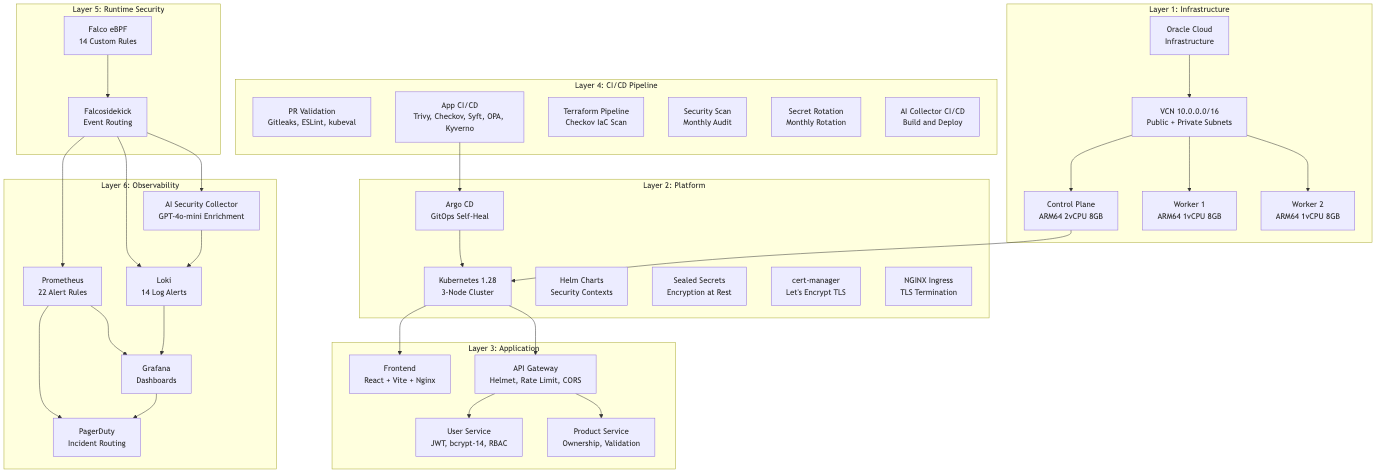
\includegraphics[width=0.85\textwidth]{../diagrams/figure-01-six-layer-architecture.png}
\caption{Six-layer Zero-Trust DevSecOps architecture, showing defence-in-depth from infrastructure through observability.}
\label{fig:arch}
\end{figure*}

\subsection{Infrastructure Layer}
The infrastructure layer is provisioned with Terraform on Oracle Cloud Infrastructure (OCI), using twelve Terraform files covering provider configuration, virtual cloud networking, subnets, route tables, security lists, gateways, and compute instances for a three-node ARM64 Kubernetes cluster (one control-plane node with a public IP, two private worker nodes reached through NAT). Hardening measures include disabling legacy Instance Metadata Service (IMDS) endpoints to mitigate SSRF-based credential theft, enabling in-transit encryption for block volumes, restricting security-list ingress to SSH (22), the Kubernetes API (6443), and required internal cluster ports, and storing Terraform state in encrypted, IAM-authenticated object storage. Checkov scans every Terraform change in CI/CD, with documented, justified exceptions.

\subsection{Platform Layer: Kubernetes and GitOps}
The platform layer separates concerns into eight namespaces (application workloads, observability, runtime security, secret management, GitOps, ingress, certificate management, and AI-augmented monitoring). Argo CD implements a bootstrap-application pattern: a single root Application resource recursively discovers every manifest under the cluster configuration directory, giving self-healing (manual cluster drift is reverted to match Git), auto-pruning (resources removed from Git are removed from the cluster), and retry-with-backoff reconciliation. The Helm chart for the application layer enforces \texttt{runAsNonRoot}, a fixed non-root UID, a read-only root filesystem, dropped Linux capabilities, and disabled privilege escalation across every workload by default.

\subsection{Application Layer}
The FreshBonds application is a four-service microservice system: a React/Vite frontend served by Nginx, an Express.js API gateway, and Express.js/MongoDB user and product services. Although the business logic is intentionally scoped for a research demonstrator, the security implementation is production-representative: Helmet-based HTTP security headers and a Content Security Policy on the gateway; bcrypt password hashing, JSON Web Tokens (JWT) with configurable expiry, minimum-length secret validation, anti-enumeration error responses, and account lockout on the user service; and role-based, ownership-scoped access control on the product service. All services share a hardened container pattern: minimal Alpine base images with packages patched at build time, a dedicated non-root user, \texttt{dumb-init} for correct signal handling, container health checks, and multi-stage builds that exclude build tooling from the runtime image.

\subsection{CI/CD Pipeline Architecture}
Six specialised GitHub Actions workflows integrate ten security tools across the delivery lifecycle (Table~\ref{tab:pipelines}, Fig.~\ref{fig:cicd}): fast pre-merge checks (linting, Gitleaks secret scanning, Kubernetes manifest validation) complete in under two minutes; a deeper application pipeline performs policy validation, container build, SBOM generation, and vulnerability scanning in eight to ten minutes; a Terraform pipeline validates and scans infrastructure changes; and monthly scheduled pipelines re-scan production images/dependencies and rotate secrets. This staged design reflects the observation that not every check needs to run on every commit: fast checks run pre-merge, comprehensive checks run on deployment, and audit checks run on a schedule.

\begin{table}[!t]
\caption{CI/CD Pipeline Summary and Security Tool Integration}
\label{tab:pipelines}
\centering
\footnotesize
\begin{tabular}{@{}p{1.5cm}p{1.0cm}p{2.9cm}@{}}
\toprule
\textbf{Pipeline} & \textbf{Duration} & \textbf{Security Tools / Blocking Gates} \\
\midrule
PR Validation & $<$2 min & ESLint, yamllint, Gitleaks, kubeval; blocks on leaked secrets or invalid manifests \\
App CI/CD & 8--10 min & OPA/Conftest, Kyverno CLI, Trivy (CVE + secret), Checkov, Syft; blocks on critical CVEs or policy violations \\
Terraform & 2--4 min & Checkov, \texttt{terraform validate}; blocks on IaC violations \\
Security Scan (monthly) & 15--20 min & Trivy, npm audit, OPA, Kyverno, Checkov; opens issue + pages on-call \\
Secret Rotation (monthly) & 3--5 min & \texttt{kubeseal}, \texttt{openssl}; rolls back on failed health check \\
AI Collector CI/CD & 5--8 min & Trivy, Syft; blocks on critical CVEs \\
\bottomrule
\end{tabular}
\end{table}

\begin{figure*}[!t]
\centering
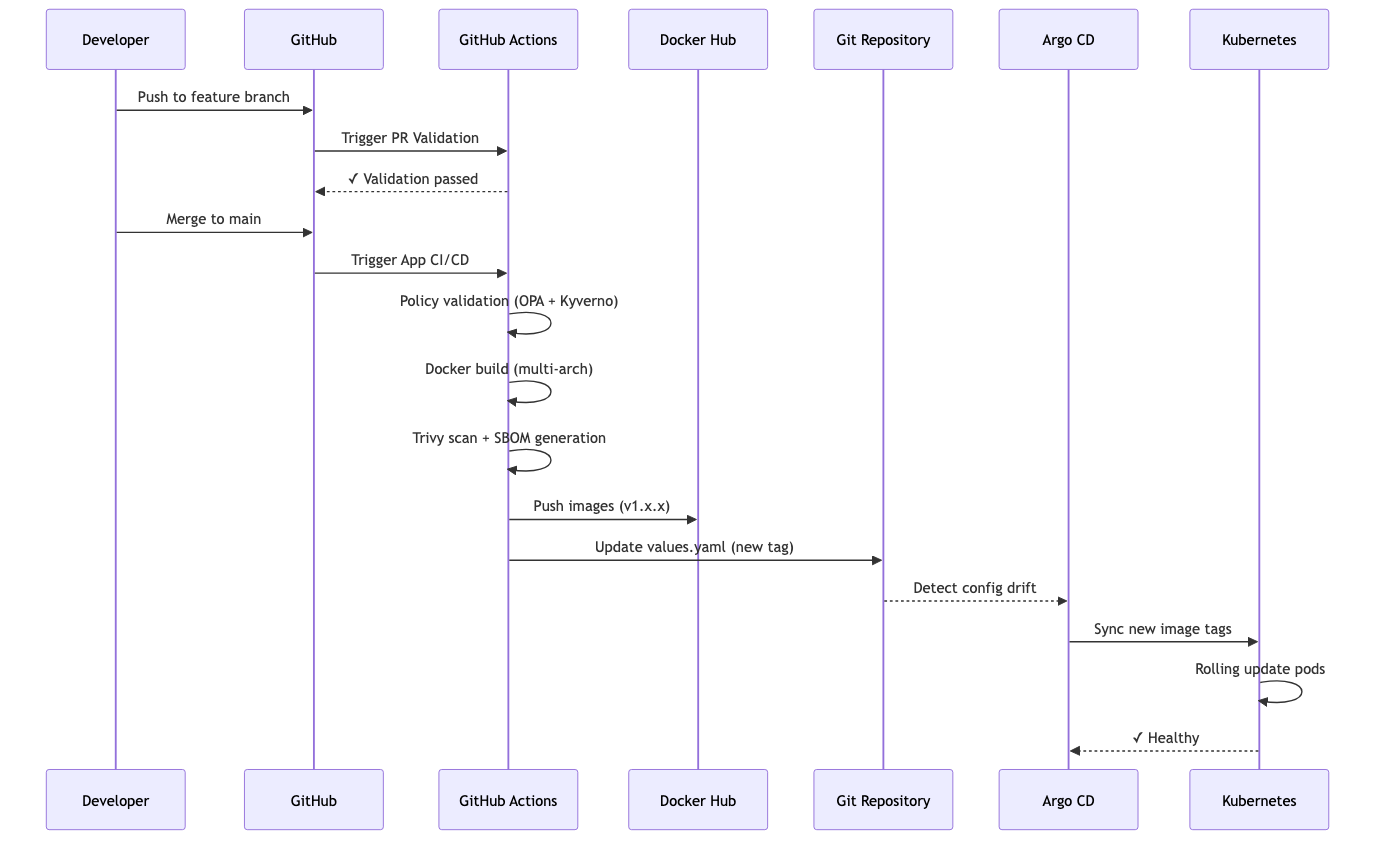
\includegraphics[width=0.85\textwidth]{../diagrams/figure-06-gitops-deployment-flow.png}
\caption{GitOps deployment flow: a merge to the main branch triggers policy validation, container build and scanning, and an SBOM-generating CI/CD pipeline, after which Argo CD detects the updated image tag and reconciles the cluster.}
\label{fig:cicd}
\end{figure*}

\subsection{Policy-as-Code Implementation}
A dual-engine design combines Kyverno and OPA. Nine Kyverno \texttt{ClusterPolicy} rules, in enforce mode, cover non-root execution, privileged-container prevention, mandatory resource limits, capability dropping, disabled privilege escalation, read-only root filesystems, prohibition of the \texttt{:latest} image tag, approved-registry enforcement, and explicit image pull policy. Sixteen OPA/Rego rules extend coverage to readiness/liveness probes, \texttt{hostPath} volume denial, dangerous-capability restriction, environment-variable credential-pattern checks, and namespace-level NetworkPolicy requirements. Both engines run in the application CI/CD pipeline (\texttt{conftest test} and \texttt{kyverno apply}) against every Kubernetes manifest, and a policy violation blocks the deployment pipeline.

\subsection{Secret Lifecycle Management}
Bitnami Sealed Secrets encrypts application secrets so that the ciphertext can be safely committed to Git; only the Sealed Secrets controller inside the target cluster, holding a private key that never leaves the cluster, can decrypt it. A monthly workflow rotates the MongoDB password (a random 32-character string applied through the database provider's administrative API), the JWT signing key (a 64-character random hex value, whose rotation invalidates all existing tokens by design, forcing re-authentication as a deliberate Zero Trust control), and payment-gateway API tokens. Every rotation is appended to a Git-committed audit log recording the timestamp, the secrets rotated, and verification status, giving an immutable, inspectable audit trail.

\subsection{Runtime Security: Falco and eBPF}
Falco runs as a Kubernetes DaemonSet using the eBPF driver for kernel-level system-call monitoring with minimal overhead. Thirteen custom rules, each mapped to a MITRE ATT\&CK for Containers technique, detect shell spawning, package-manager execution, cryptocurrency-mining process signatures, sensitive-file reads, \texttt{setuid} privilege escalation, reverse shells, container-escape attempts (\texttt{nsenter}, \texttt{runc}, \texttt{crictl}), connections to known attacker ports, tampering with system files such as \texttt{/etc/passwd}, network reconnaissance tooling, suspicious DNS query patterns, and large outbound data transfers. Matched events are forwarded through Falcosidekick to Prometheus Alertmanager, PagerDuty, and an AI Security Collector simultaneously (Fig.~\ref{fig:runtime}), so that the primary alerting path never depends on the availability of the AI component.

\begin{figure*}[!t]
\centering
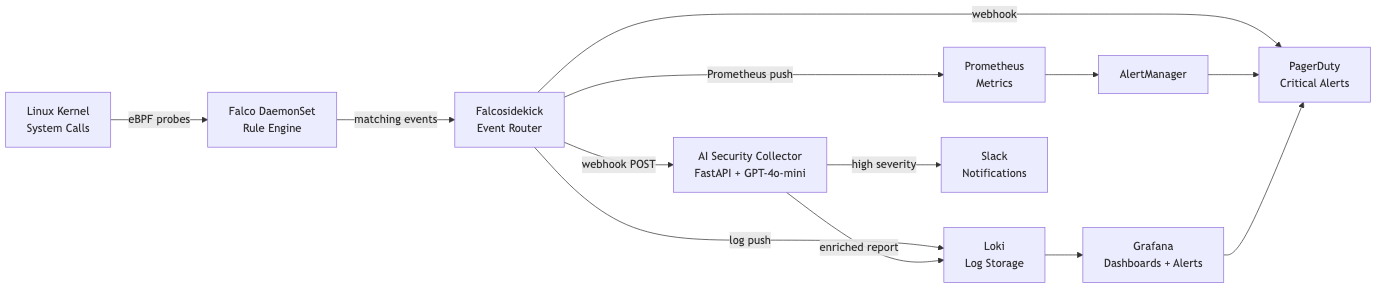
\includegraphics[width=0.85\textwidth]{../diagrams/figure-09-runtime-security-flow.png}
\caption{Runtime security event flow: Falco events fan out to Alertmanager/PagerDuty (primary alert path) and to the AI Security Collector for enrichment and storage, independently of one another.}
\label{fig:runtime}
\end{figure*}

\subsection{Observability Stack}
A three-pillar observability model combines Prometheus metrics, Loki logs, and Alertmanager/Grafana alerting. Twenty-two Prometheus alert rules cover infrastructure health (disk, memory, node readiness), application health (service availability, latency, crash-looping, out-of-memory kills), and Falco self-monitoring (daemon availability, event-rate anomalies, dropped-event detection). Fourteen Grafana/Loki rules add log-based detection of application errors, MongoDB connectivity loss, and login-security anomalies such as brute-force and account-enumeration patterns. Alertmanager applies two-tier routing, escalating critical alerts to PagerDuty immediately and routing warnings through a standard notification policy.

\subsection{AI-Augmented Security Monitoring}
An AI Security Collector, implemented as a FastAPI service, receives Falco events from Falcosidekick over a webhook, persists them to Loki (with a local JSONL fallback if Loki is unavailable), deduplicates repeated events, and -- for high-severity events, and only when Azure OpenAI credentials are configured -- queues a GPT-4o-mini-generated report describing the likely threat, recommended investigation steps, and remediation actions. Delivery integrations exist for Slack, PagerDuty, and generic webhooks. Because the collector consumes events from the same fan-out as Alertmanager rather than sitting in front of it, AI enrichment can fail, degrade, or be disabled entirely without affecting the primary detection and alerting path.

\section{Evaluation}

\subsection{Evaluation Methodology}
Consistent with design-science evaluation guidance \cite{hevner2004}, the framework is evaluated primarily through repository and artefact investigation, complemented by controlled fault-injection experiments. Five evaluation experiments were conducted: (E1) repository structure verification against the intended architecture; (E2) security-control coverage analysis, counting and classifying Kyverno, OPA, Falco, and Prometheus rules; (E3) CI/CD gate analysis, tracing where insecure changes are blocked or reported; (E4) runtime response-path analysis, tracing an injected event from Falco through Falcosidekick to Alertmanager, PagerDuty, Loki, and AI enrichment; and (E5) NIST SP 800-207 tenet mapping against implementation evidence.

\subsection{NIST SP 800-207 Zero Trust Compliance Mapping}
Table~\ref{tab:nist} maps each of the seven NIST tenets to concrete implementation evidence. All seven tenets are assessed as strongly satisfied: every Kubernetes object is individually secured and version-controlled; ingress traffic is terminated over TLS via cert-manager and Let's Encrypt while the database connection enforces TLS; API access uses short-lived JWTs verified on every request; policy is enforced dynamically by Kyverno, OPA, and Falco without requiring service restarts; Trivy, Checkov, npm audit, Prometheus, Loki, and Falco continuously monitor asset integrity; JWT validation, ownership middleware, RBAC, and security contexts strictly gate access; and workflow artefacts, SBOMs, rotation logs, and Falco/Loki events feed back into an evidence trail that supports posture improvement.

\begin{table*}[!t]
\caption{NIST SP 800-207 Zero Trust Tenet Compliance Mapping}
\label{tab:nist}
\centering
\footnotesize
\begin{tabular}{@{}p{4.3cm}p{11.5cm}c@{}}
\toprule
\textbf{NIST ZTA Tenet} & \textbf{Implementation Evidence} & \textbf{Assessment} \\
\midrule
All data sources and computing services are resources & Every pod, service, secret, image, infrastructure object, and workflow has its own security context, credentials, and access policy & Strong \\
All communication is secured regardless of network location & TLS termination at ingress (cert-manager/Let's Encrypt); TLS-only database connections; internal traffic addressed via ClusterIP services & Strong \\
Access is granted per session & JWTs with an 8-hour expiry, verified on every request; no persistent sessions; per-request ownership checks & Strong \\
Access is determined by dynamic policy & Kyverno (9 rules), OPA (16 rules), and Falco (13--14 rules) enforce policy across admission, CI/CD, and runtime without service restarts & Strong \\
Integrity and security posture are continuously monitored & Prometheus (22 alerts), Falco (13--14 rules), Trivy, Checkov, and npm audit continuously assess asset posture & Strong \\
Authentication and authorisation are strictly enforced before access & JWT validation, RBAC, ownership middleware, and Kubernetes security contexts gate every access path & Strong \\
Asset and network state is collected to improve security posture & Workflow artefacts, SARIF/SBOM outputs, rotation logs, and Falco/Loki events form a continuous feedback loop & Strong \\
\bottomrule
\end{tabular}
\end{table*}

\subsection{Pipeline Security Gate Effectiveness}
To validate blocking behaviour empirically, a container image containing a known critical-severity vulnerability was intentionally introduced at the build stage. Trivy identified the vulnerability and failed the pipeline, preventing the image from being deployed to the cluster. Separately, a non-compliant manifest (a privileged container with no resource limits) was submitted for validation; both Kyverno and OPA independently rejected it at the admission-control stage. These two experiments confirm that the CI/CD and admission-time gates summarised in Table~\ref{tab:pipelines} behave as designed rather than merely reporting findings without consequence.

\subsection{Policy Enforcement Coverage Analysis}
Table~\ref{tab:coverage} distributes the thirty-nine policy and runtime rules across ten security domains. Kyverno and OPA together dominate deployment-time domains (container privilege, resource management, image security, capability restriction), while Falco supplies the only coverage for domains that are only observable at runtime: execution control, credential access at runtime, and data-exfiltration behaviour. This distribution is the direct evidence for the defence-in-depth design principle: no single engine covers every domain.

\begin{table}[!t]
\caption{Policy Enforcement Coverage by Security Domain}
\label{tab:coverage}
\centering
\footnotesize
\begin{tabular}{@{}p{2.1cm}ccc c@{}}
\toprule
\textbf{Security Domain} & \textbf{Kyverno} & \textbf{OPA} & \textbf{Falco} & \textbf{Total} \\
\midrule
Container privilege & 3 & 3 & 2 & 8 \\
Resource management & 1 & 1 & 0 & 2 \\
Image security & 3 & 2 & 0 & 5 \\
Filesystem security & 1 & 1 & 2 & 4 \\
Capability restriction & 1 & 2 & 0 & 3 \\
Network security & 0 & 3 & 3 & 6 \\
Credential protection & 0 & 0 & 2 & 2 \\
Health monitoring & 0 & 2 & 0 & 2 \\
Execution control & 0 & 0 & 3 & 3 \\
Data protection & 0 & 0 & 2 & 2 \\
\midrule
\textbf{Total} & \textbf{9} & \textbf{16} & \textbf{14} & \textbf{39} \\
\bottomrule
\end{tabular}
\end{table}

\subsection{Runtime Detection and MITRE ATT\&CK Coverage}
A controlled runtime test modified \texttt{/etc/hosts} inside a test pod to simulate unauthorised file tampering. Falco raised a critical-severity alert within one second, which was forwarded through Falcosidekick to the AI Security Collector and, with AI enrichment enabled, produced a contextual incident report. Table~\ref{tab:mitre} maps the thirteen custom Falco rules onto the MITRE ATT\&CK for Containers matrix: coverage spans eight of the twelve tactics (Execution, Persistence, Privilege Escalation, Credential Access, Discovery, Command and Control, Exfiltration, and Impact), with the strongest coverage concentrated in Execution, Privilege Escalation, Credential Access, and Command and Control -- the tactics most frequently observed in real container-compromise incidents. Initial Access is intentionally out of scope (it precedes the container boundary), and Defence Evasion, Lateral Movement, and Collection are only partially covered through built-in Falco rules and NetworkPolicy segmentation rather than the custom rule set. Detection latency measured at the eBPF layer was under one second for most categories and under thirty seconds for threshold-based data-exfiltration detection.

\begin{table}[!t]
\caption{MITRE ATT\&CK for Containers Coverage}
\label{tab:mitre}
\centering
\footnotesize
\begin{tabular}{@{}p{2.3cm}p{2.9cm}c@{}}
\toprule
\textbf{Tactic} & \textbf{Representative Technique(s)} & \textbf{Rules} \\
\midrule
Execution & T1059, T1059.004 & 2 \\
Persistence & T1546, T1543 & 2 \\
Privilege Escalation & T1548, T1611 & 2 \\
Credential Access & T1552, T1552.001 & 2 \\
Discovery & T1046 & 1 \\
Command and Control & T1571, T1071.004 & 2 \\
Exfiltration & T1048 & 1 \\
Impact & T1496 & 1 \\
\bottomrule
\end{tabular}
\end{table}

\subsection{Supply Chain Security and Compliance Summary}
Supply-chain controls span container and dependency vulnerability scanning (Trivy, npm audit), dual-format SBOM generation (SPDX and CycloneDX, satisfying both government and OWASP-aligned tooling requirements), Git secret scanning (Gitleaks), infrastructure-as-code scanning (Checkov), and registry/tag governance (Kyverno approved-registry and no-\texttt{latest}-tag rules). Table~\ref{tab:metrics} consolidates the key compliance metrics produced across all evaluation experiments.

\begin{table}[!t]
\caption{Compliance Metrics Summary}
\label{tab:metrics}
\centering
\footnotesize
\begin{tabular}{@{}p{3.3cm}p{1.6cm}@{}}
\toprule
\textbf{Metric} & \textbf{Value} \\
\midrule
NIST SP 800-207 tenets satisfied & 7 / 7 \\
Total policy and runtime rules & 39 \\
CI/CD security tools integrated & 10 \\
CI/CD pipelines & 6 \\
Prometheus alert rules & 22 \\
Grafana/Loki alert rules & 14 \\
MITRE ATT\&CK techniques covered & 13 \\
MITRE ATT\&CK tactics covered & 8 / 12 \\
SBOM formats generated & 2 (SPDX, CycloneDX) \\
Critical-CVE deployments blocked (tested) & All tested cases \\
Maximum measured runtime detection latency & $<$30 s \\
Secret rotation frequency & Monthly, automated \\
\bottomrule
\end{tabular}
\end{table}

\section{Discussion}

\subsection{Critical Analysis}
The framework's principal strength is integration rather than any individual tool: Trivy's SARIF output feeds GitHub code scanning, Falco events fan out simultaneously to Prometheus, Loki, PagerDuty, and the AI collector, and secret-rotation commits trigger an Argo CD sync that updates running pods automatically, so a security event at any layer becomes visible across the whole observability stack. Because every infrastructure, policy, and (encrypted) secret change is committed to Git, the repository itself functions as an immutable audit log, turning compliance verification into Git-history inspection rather than live interrogation.

Three trade-offs qualify these results. First, Kubernetes-native policy validation currently runs primarily through the Kyverno CLI inside CI/CD rather than as an in-cluster admission webhook, so a resource applied directly to the cluster outside the pipeline would bypass policy checks -- a scope limitation rather than a design flaw, and one identified explicitly as future work. Second, the framework has not been subjected to formal red-team or adversarial-simulation testing; the MITRE ATT\&CK mapping demonstrates rule-level technique coverage, not measured detection precision or recall against an adaptive adversary. Third, the AI Security Collector depends on an external LLM API and is subject to hallucination risk; the non-blocking architecture bounds the operational impact of this dependency but does not eliminate the need for human review of AI-generated reports.

\subsection{Comparison with Existing Approaches}
Table~\ref{tab:comparison} situates this work against the conceptual and guideline-level references it builds on. Unlike NIST SP 800-207 and the DoD Zero Trust Reference Architecture, which define tenets and pillars but not an implementation, or OWASP's DevSecOps guideline, which is pipeline-focused and does not address runtime detection, this framework demonstrates a working, evaluated system spanning six layers with two policy engines, eBPF-based runtime detection, dual-format SBOMs, automated secret rotation, and AI-based enrichment -- evaluated jointly against NIST tenets and MITRE ATT\&CK technique coverage.

\begin{table}[!t]
\caption{Comparison with Existing Approaches}
\label{tab:comparison}
\centering
\footnotesize
\begin{tabular}{@{}p{1.6cm}p{1.5cm}p{1.5cm}p{1.4cm}@{}}
\toprule
\textbf{Aspect} & \textbf{This Work} & \textbf{NIST 800-207 \cite{rose2020}} & \textbf{OWASP DevSecOps \cite{owasp2023}} \\
\midrule
Type & Implementation & Reference architecture & Guideline \\
Policy engines & 2 (Kyverno + OPA) & Not specified & OPA recommended \\
Runtime security & Falco/eBPF, 13 rules & Tenet only & Not addressed \\
AI integration & GPT-4o-mini enrichment & Not addressed & Not addressed \\
Evaluation & NIST + MITRE mapping & N/A & N/A \\
\bottomrule
\end{tabular}
\end{table}

\subsection{Limitations and Threats to Validity}
\emph{Internal validity:} the evaluation relies primarily on repository evidence and controlled fault injection rather than sustained adversarial testing, and the NIST/MITRE mappings reflect the authors' interpretation, which other reviewers might assess differently. \emph{External validity:} the framework runs on a single three-node OCI cluster with a purpose-built demonstration application; scalability to larger, multi-cluster, multi-cloud, or higher-complexity production estates has not been validated. \emph{Construct validity:} rule and tool-integration counts are used as coverage proxies, but count does not equal quality -- rule specificity and false-positive rate matter and are not measured here. Specific, acknowledged limitations include the absence of formal red-team evaluation, service-mesh mutual TLS, quantitative pipeline/runtime performance benchmarking, cryptographic image-signature verification, and a unit/integration test suite for the microservices.

\section{Conclusion and Future Work}

This paper presented the design, implementation, and evaluation of a Zero-Trust DevSecOps framework for Kubernetes-based microservices. The six-layer architecture integrates infrastructure-as-code, GitOps deployment, dual-engine policy-as-code enforcement, container and dependency scanning with dual-format SBOM generation, automated secret rotation, eBPF-based runtime detection, and non-blocking AI-assisted incident enrichment into a single, reproducible pipeline deployed on a production-grade Kubernetes cluster. Evaluation confirms alignment with all seven NIST SP 800-207 Zero Trust tenets, enforcement of thirty-nine policy and runtime rules across ten security domains, coverage of thirteen MITRE ATT\&CK for Containers techniques across eight of twelve tactics, and empirically verified blocking behaviour at both CI/CD and admission-control gates. The central finding is that continuous compliance is best understood as a property of the delivery lifecycle rather than of any single tool or periodic audit: it emerges from automated control points distributed before merge, before deployment, after deployment, and during runtime operation.

Future work follows directly from the limitations identified in Section VI-C: deploying Kyverno as an in-cluster admission webhook to close the CI/CD-bypass gap; conducting formal, MITRE ATT\&CK-mapped red-team evaluation to measure detection precision and recall under adversarial conditions; extending the architecture to multi-cluster and multi-cloud deployments; adding service-mesh mutual TLS for internal traffic; integrating Sigstore/Cosign image-signature verification with Kyverno-enforced admission checks; and training anomaly-detection models (for example, isolation forests, autoencoders, or sequence models) on collected Falco and Prometheus telemetry to complement the current rule-based detection with learned, adaptive detection. The complete implementation, including infrastructure definitions, CI/CD workflows, policy specifications, and the AI Security Collector, is released as an open-source reference implementation to support reproduction and extension by other researchers and practitioners.

\section*{Acknowledgment}
The author thanks the supervisor, Roshan N. Rajapakse, and the lecturers and peers at the University of Colombo School of Computing for their guidance and feedback throughout this work, and acknowledges the maintainers and communities of the open-source projects used in the implementation, including Kubernetes, Open Policy Agent, Kyverno, Falco, Trivy, Checkov, Syft, Sealed Secrets, Prometheus, Grafana, Loki, Argo CD, and Terraform. The author also acknowledges Oracle for Always Free Tier cloud infrastructure credits and Microsoft for Azure OpenAI Service credits used during the AI-augmented monitoring evaluation.

\begin{thebibliography}{00}

\bibitem{cncf2024} Cloud Native Computing Foundation, ``CNCF Annual Survey 2024,'' 2024. [Online]. Available: https://www.cncf.io/reports/

\bibitem{burns2016} B. Burns, B. Grant, D. Oppenheimer, E. Brewer, and J. Wilkes, ``Borg, Omega, and Kubernetes: lessons learned from three container-management systems over a decade,'' \emph{ACM Queue}, vol. 14, no. 1, pp. 70--93, 2016.

\bibitem{kindervag2010} J. Kindervag, ``Build security into your network's DNA: the Zero Trust network architecture,'' Forrester Research, 2010.

\bibitem{sonatype2023} Sonatype Inc., ``9th Annual State of the Software Supply Chain Report,'' 2023.

\bibitem{redhat2024} Red Hat, ``The State of Kubernetes Security Report 2024,'' 2024. [Online]. Available: https://www.redhat.com/en/resources/state-kubernetes-security-report

\bibitem{rose2020} S. Rose, O. Borchert, S. Mitchell, and S. Connelly, ``Zero Trust Architecture,'' NIST Special Publication 800-207, National Institute of Standards and Technology, Gaithersburg, MD, 2020.

\bibitem{myrbakken2017} H. Myrbakken and R. Colomo-Palacios, ``DevSecOps: a multivocal literature review,'' in \emph{Software Process Improvement and Capability Determination}. Cham: Springer, 2017, pp. 17--29.

\bibitem{hevner2004} A. R. Hevner, S. T. March, J. Park, and S. Ram, ``Design science in information systems research,'' \emph{MIS Quarterly}, vol. 28, no. 1, pp. 75--105, 2004.

\bibitem{peffers2007} K. Peffers, T. Tuunanen, M. A. Rothenberger, and S. Chatterjee, ``A design science research methodology for information systems research,'' \emph{Journal of Management Information Systems}, vol. 24, no. 3, pp. 45--77, 2007.

\bibitem{biden2021} J. R. Biden, ``Executive Order 14028: Improving the Nation's Cybersecurity,'' \emph{Federal Register}, vol. 86, no. 93, pp. 26633--26647, 2021.

\bibitem{disa2021} Defense Information Systems Agency, ``Department of Defense Zero Trust Reference Architecture,'' 2021.

\bibitem{owasp2023} OWASP, ``OWASP DevSecOps Guideline,'' 2023. [Online]. Available: https://owasp.org/www-project-devsecops-guideline/

\bibitem{souppaya2022} M. Souppaya, K. Scarfone, and D. Dodson, ``Secure software development framework (SSDF) version 1.1,'' NIST Special Publication 800-218, National Institute of Standards and Technology, Gaithersburg, MD, 2022.

\bibitem{fitzgerald2017} B. Fitzgerald and K.-J. Stol, ``Continuous software engineering: a roadmap and agenda,'' \emph{Journal of Systems and Software}, vol. 123, pp. 176--189, 2017.

\bibitem{jeyaraj2023} A. Jeyaraj, ``Zero trust security in cloud-native environments: challenges and implementation strategies,'' \emph{Journal of Cloud Computing}, vol. 12, no. 1, pp. 1--18, 2023.

\bibitem{sanchez2020} S. Sanchez-Gordon and R. Colomo-Palacios, ``Security as code: a systematic mapping study,'' in \emph{Int. Conf. on Computational Science and Its Applications}. Cham: Springer, 2020, pp. 159--174.

\bibitem{kubernetes2024} Kubernetes, ``Kubernetes Documentation: Pod Security Standards,'' 2024. [Online]. Available: https://kubernetes.io/docs/concepts/security/pod-security-standards/

\bibitem{cis2024} Center for Internet Security, ``CIS Kubernetes Benchmark v1.8,'' 2024.

\bibitem{shamim2020} M. S. Shamim, F. A. Bhuiyan, and A. Rahman, ``XI commandments of Kubernetes security: a systematization of knowledge related to Kubernetes security practices,'' in \emph{IEEE Secure Development Conf. (SecDev)}, 2020, pp. 58--64.

\bibitem{opa2024} Open Policy Agent, ``Open Policy Agent Documentation,'' 2024. [Online]. Available: https://www.openpolicyagent.org/

\bibitem{kyverno2024} Kyverno, ``Kyverno: Kubernetes Native Policy Management,'' 2024. [Online]. Available: https://kyverno.io/

\bibitem{aqua2024} Aqua Security, ``Trivy: a comprehensive and versatile security scanner,'' 2024. [Online]. Available: https://trivy.dev/

\bibitem{anchore2026} Anchore, ``Syft Documentation,'' 2026. [Online]. Available: https://github.com/anchore/syft

\bibitem{bridgecrew2024} Bridgecrew, ``Checkov: policy-as-code for everyone,'' 2024. [Online]. Available: https://www.checkov.io/

\bibitem{souppaya2023} M. Souppaya, J. Morello, and K. Scarfone, ``Strategies for the integration of software supply chain security in DevSecOps CI/CD pipelines,'' NIST Special Publication 800-204C, National Institute of Standards and Technology, Gaithersburg, MD, 2023.

\bibitem{falco2024} The Falco Project, ``Falco: cloud-native runtime security,'' 2024. [Online]. Available: https://falco.org/

\bibitem{rice2022} L. Rice, \emph{Learning eBPF: Programming the Linux Kernel for Enhanced Observability, Networking, and Security}. Sebastopol, CA: O'Reilly Media, 2022.

\bibitem{mitre2024} MITRE, ``ATT\&CK for Containers,'' 2024. [Online]. Available: https://attack.mitre.org/matrices/enterprise/containers/

\bibitem{alahmadi2020} B. A. Alahmadi, L. Axon, and T. Sherren, ``99\% false positives: a qualitative study of SOC analysts' perspectives on security alarms,'' in \emph{Proc. USENIX Security Symposium}, 2020, pp. 2203--2220.

\bibitem{microsoft2024} Microsoft, ``Azure OpenAI Service Documentation,'' 2024. [Online]. Available: https://learn.microsoft.com/azure/ai-services/openai/

\bibitem{cloudsecurityalliance2022} Cloud Security Alliance, ``DevSecOps: integrating security into DevOps,'' CSA Working Group Publication, 2022.

\bibitem{pcissc2022} PCI Security Standards Council, ``PCI DSS v4.0: Payment Card Industry Data Security Standard,'' 2022.

\end{thebibliography}

\end{document}
